\section{Baseline Experiments}
\label{sec:experiments}

\subsection{Experimental Setup}
\label{ssec:exp_setup}

We evaluate six representative state-of-the-art vision-language models on the four
\lucid{} benchmark tasks. All models are evaluated in a zero-shot setting using
standardised prompt templates, with no fine-tuning on \lucid{} training data.
Experiments were run on a cluster of 32 NVIDIA A100 (80~GB) GPUs. For models with
open weights (LLaVA-1.6, BLIP-2, InstructBLIP, LLaMA-3.2V), inference was conducted
using HuggingFace Transformers~\cite{wolf2020transformers} with bfloat16 precision.
API-based models (GPT-4V) were queried via the official inference endpoint.

\paragraph{Models evaluated.}
\begin{itemize}[leftmargin=2em, noitemsep]
  \item \textbf{GPT-4V}~\cite{openai2023gpt4}: OpenAI's GPT-4 with vision, queried
        with 8 images per call maximum.
  \item \textbf{DriveLM-Agent}~\cite{sima2023drivelm}: A DriveLM fine-tuned LLaMA-7B
        variant specialised for driving VQA chains.
  \item \textbf{LLaMA-3.2-Vision (11B)}~\cite{meta2024llama3}: Meta's multimodal
        extension of LLaMA 3.2 with native visual understanding.
  \item \textbf{LLaVA-1.6 (13B)}~\cite{liu2023visual}: A visual instruction-tuned model
        based on Mistral-7B with LLaVA-NeXT improvements.
  \item \textbf{InstructBLIP (13B)}~\cite{dai2023instructblip}: BLIP-2 with
        instruction-tuned language decoder (Vicuna-13B).
  \item \textbf{BLIP-2 (OPT-6.7B)}~\cite{li2023blip2}: Bootstrapped language-image
        pre-training with Q-Former architecture.
\end{itemize}

\subsection{Results: Causal Scene Understanding (CSU)}
\label{ssec:exp_csu}

\begin{table}[htbp]
  \centering
  \caption{Results on the Causal Scene Understanding (CSU) task.
  All models evaluated zero-shot on the \lucid{} test split.}
  \label{tab:csu_results}
  \small
  \begin{tabular}{lcccccc}
    \toprule
    \textbf{Model} & \textbf{BLEU-4} & \textbf{CIDEr} & \textbf{METEOR} & \textbf{BERTScore} & \textbf{Human Eval} \\
    \midrule
    GPT-4V           & \textbf{18.4} & \textbf{82.3} & \textbf{24.7} & \textbf{0.812} & \textbf{4.1/5} \\
    DriveLM-Agent    & 16.7 & 75.4 & 22.8 & 0.797 & 3.9/5 \\
    LLaMA-3.2V       & 15.1 & 69.8 & 21.4 & 0.781 & 3.7/5 \\
    LLaVA-1.6        & 14.2 & 64.1 & 20.3 & 0.773 & 3.6/5 \\
    InstructBLIP     & 12.3 & 58.9 & 19.1 & 0.752 & 3.4/5 \\
    BLIP-2           & 10.8 & 51.7 & 17.6 & 0.731 & 3.2/5 \\
    \midrule
    \multicolumn{6}{l}{\textit{Difficulty-stratified (GPT-4V):}} \\
    ~~ Easy (chain $\le 3$)    & 26.3 & 112.4 & 31.8 & 0.851 & 4.4/5 \\
    ~~ Medium (chain 4--7)     & 18.7 & 84.1  & 24.9 & 0.813 & 4.1/5 \\
    ~~ Hard (chain $\ge 8$)    & 10.1 & 48.7  & 16.2 & 0.762 & 3.6/5 \\
    \bottomrule
  \end{tabular}
\end{table}

GPT-4V achieves the highest scores across all metrics, followed by the AD-specialised
DriveLM-Agent which benefits from task-relevant pre-training. The significant
drop from Easy to Hard difficulty (BLEU-4: 26.3 $\to$ 10.1) confirms that long causal
chains genuinely challenge current models, validating the difficulty stratification.

\subsection{Results: Counterfactual Reasoning (CFR)}
\label{ssec:exp_cfr}

\begin{table}[htbp]
  \centering
  \caption{Results on the Counterfactual Reasoning (CFR) task (multiple choice).}
  \label{tab:cfr_results}
  \small
  \begin{tabular}{lcccc}
    \toprule
    \textbf{Model} & \textbf{Accuracy (\%)} & \textbf{Macro-F1} & \textbf{Consistency (\%)} \\
    \midrule
    GPT-4V           & \textbf{58.3} & \textbf{61.2} & \textbf{72.4} \\
    DriveLM-Agent    & 52.1 & 55.8 & 68.7 \\
    LLaMA-3.2V       & 48.6 & 51.3 & 65.1 \\
    LLaVA-1.6        & 44.7 & 47.8 & 61.3 \\
    InstructBLIP     & 41.9 & 44.7 & 58.2 \\
    BLIP-2           & 38.2 & 41.4 & 54.6 \\
    Random baseline  & 33.3 & 33.3 & -- \\
    \bottomrule
  \end{tabular}
\end{table}

All models perform only modestly above the 33.3\% random baseline, with the best
model (GPT-4V) reaching 58.3\%. Consistency scores are notably lower than accuracy
for all models, indicating that models frequently give mutually contradictory answers
to paired counterfactual questions. This confirms that counterfactual consistency ---
a prerequisite for trustworthy causal reasoning --- is not reliably achieved by any
current model.

\subsection{Results: Instruction-following Navigation (IFN)}
\label{ssec:exp_ifn}

\begin{table}[htbp]
  \centering
  \caption{Results on the Instruction-following Navigation (IFN) task.}
  \label{tab:ifn_results}
  \small
  \begin{tabular}{lcccc}
    \toprule
    \textbf{Model} & \textbf{ISR (\%)} & \textbf{Path Quality (ADE$\downarrow$)} & \textbf{Report BLEU-4} \\
    \midrule
    GPT-4V           & \textbf{42.7} & \textbf{1.83} & \textbf{19.3} \\
    DriveLM-Agent    & 38.9 & 2.14 & 17.6 \\
    LLaMA-3.2V       & 35.7 & 2.47 & 16.2 \\
    LLaVA-1.6        & 32.4 & 2.81 & 14.8 \\
    InstructBLIP     & 29.3 & 3.12 & 13.1 \\
    BLIP-2           & 25.8 & 3.74 & 11.2 \\
    \bottomrule
  \end{tabular}
\end{table}

The best ISR of 42.7\% (GPT-4V) indicates that current models fail to successfully
follow navigation instructions in the majority of test cases, pointing to a
fundamental gap in language-conditioned trajectory generation. Failure analysis
reveals that the most common errors are: (1) ignoring speed constraints specified
in the instruction (38.2\% of failures); (2) incorrect lane assignment (29.7\%);
and (3) misidentification of the referenced agent (\eg{} wrong pedestrian) (21.4\%).

\subsection{Results: Risk-Aware Planning (RAP)}
\label{ssec:exp_rap}

\begin{table}[htbp]
  \centering
  \caption{Results on the Risk-Aware Planning (RAP) task.}
  \label{tab:rap_results}
  \small
  \begin{tabular}{lcccc}
    \toprule
    \textbf{Model} & \textbf{CAR (\%)} & \textbf{Risk MAE$\downarrow$} & \textbf{Action Acc.\ (\%)} & \textbf{EQ (Human)} \\
    \midrule
    GPT-4V           & \textbf{78.3} & \textbf{0.74} & \textbf{61.8} & \textbf{4.2/5} \\
    DriveLM-Agent    & 72.4 & 0.88 & 57.3 & 4.0/5 \\
    LLaMA-3.2V       & 68.1 & 1.02 & 53.7 & 3.8/5 \\
    LLaVA-1.6        & 63.7 & 1.17 & 49.2 & 3.5/5 \\
    InstructBLIP     & 58.9 & 1.31 & 45.6 & 3.2/5 \\
    BLIP-2           & 54.2 & 1.48 & 41.3 & 3.0/5 \\
    \bottomrule
  \end{tabular}
\end{table}

\begin{figure}[htbp]
  \centering
  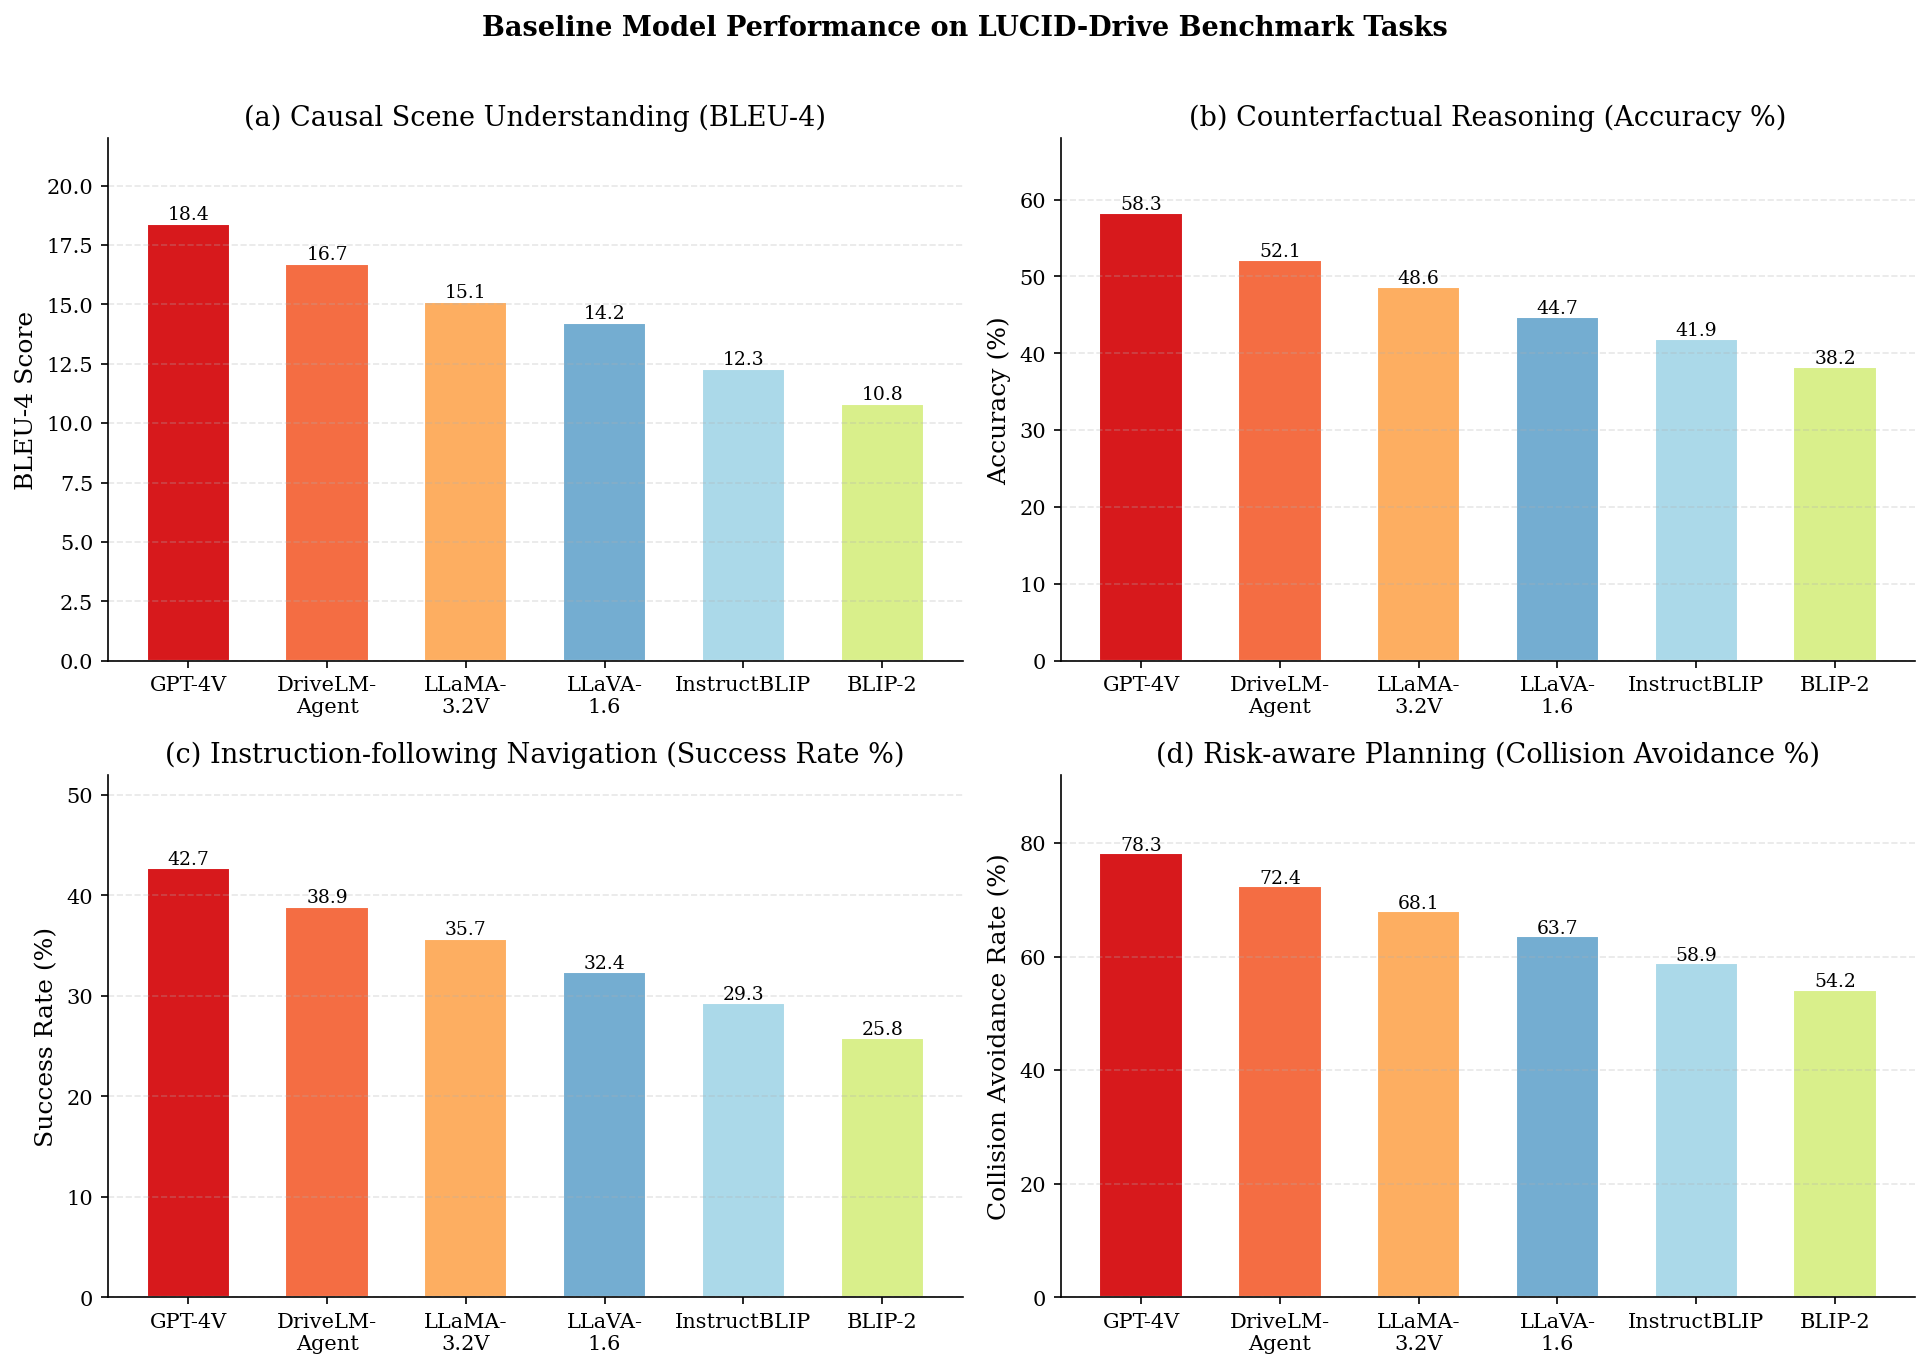
\includegraphics[width=\linewidth]{figures/baseline_results.png}
  \caption{Summary of baseline model performance across the four \lucid{} benchmark tasks:
  (a) CSU (BLEU-4), (b) CFR (Accuracy \%), (c) IFN (Success Rate \%), (d) RAP
  (Collision Avoidance \%). GPT-4V leads across all tasks; all models leave
  substantial room for improvement, validating the difficulty of \lucid{}.}
  \label{fig:baseline_results}
\end{figure}

RAP results reveal that risk awareness is comparatively stronger than pure
counterfactual reasoning: GPT-4V achieves 78.3\% CAR, suggesting that broad
commonsense safety knowledge provides a reasonable foundation for risk avoidance.
However, action-level accuracy (61.8\%) and risk severity MAE (0.74) indicate that
models still struggle with precise risk quantification and optimal action selection.

\subsection{Error Analysis and Failure Modes}
\label{ssec:exp_errors}

We conducted a qualitative error analysis on 200 randomly sampled incorrect
predictions from the CFR and IFN tasks. Key failure modes include:

\begin{enumerate}[leftmargin=2em, noitemsep]
  \item \textbf{Temporal grounding failures}: Models fail to correctly anchor causal
        events to the right temporal position in a multi-frame sequence (32.4\% of
        CFR errors).
  \item \textbf{Counterfactual inconsistency}: Answers to paired counterfactuals
        logically contradict each other, indicating that models generate answers
        independently rather than through genuine hypothetical simulation (27.8\% of
        CFR errors).
  \item \textbf{Agent confusion in crowded scenes}: In scenarios with many similar
        agents (\eg{} multiple cyclists), models confuse the causal agent referenced
        in the question (18.3\% of CSU and IFN errors).
  \item \textbf{Instruction over-simplification}: Models follow only the first clause
        of multi-clause instructions, ignoring compound constraints (22.1\% of IFN
        errors).
  \item \textbf{Adverse-condition hallucination}: Under fog or night conditions,
        models sometimes hallucinate objects that are not visible in the images,
        likely due to prior-driven confabulation (14.7\% of RAP errors).
\end{enumerate}

These findings highlight concrete directions for future model improvement and
confirm that \lucid{} provides a challenging, discriminative evaluation framework.
